\section{Implementation}\label{sec:03_impl}
% Explain section
This section explains the implementation based on the conceptual design introduced in \Sec{sec:02_design}. 
% MVC
As mentioned in \Sec{sec:01_intro}, the MVC architecture is used to implement this application. \Fig{fig:03_impl_structure} presents the project folder structure of the MVC implementation.
% What is what
The models are introduced in \Sec{subsec:03_impl_models}, the views, and controllers in \Sec{subsec:03_impl_servlets}.
% Others
Additionally, this implementation uses custom object stores (introduced in \Sec{subsec:03_impl_objstores}) and filters (introduced in \Sec{subsec:03_impl_filters}).
% Figure
\begin{figure}[h]
\centering
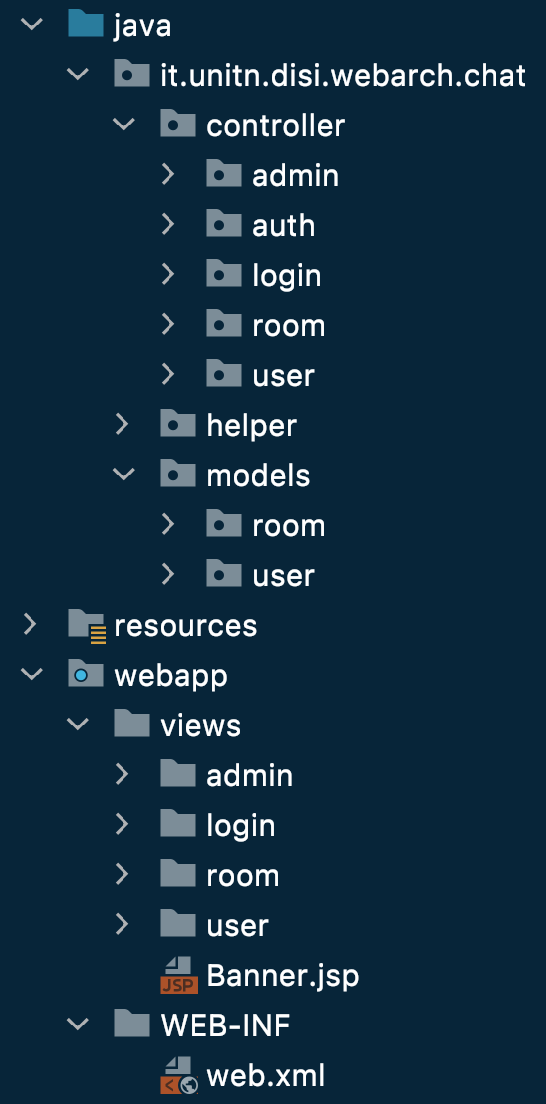
\includegraphics[scale=0.5]{images/03_impl/structure}
\caption{Project folder structure}
\label{fig:03_impl_structure}
\end{figure}


\subsection{Models}\label{subsec:03_impl_models}
% Intro
As being mentioned, this project is implemented using the MVC pattern. Therefore, each entity of the chat system is represented by a model.
% Beans
Each model is implemented using the Java Bean specification. This enables to reuse the models in \texttt{JSP} files.
% Figure
\begin{figure}[h]
\centering
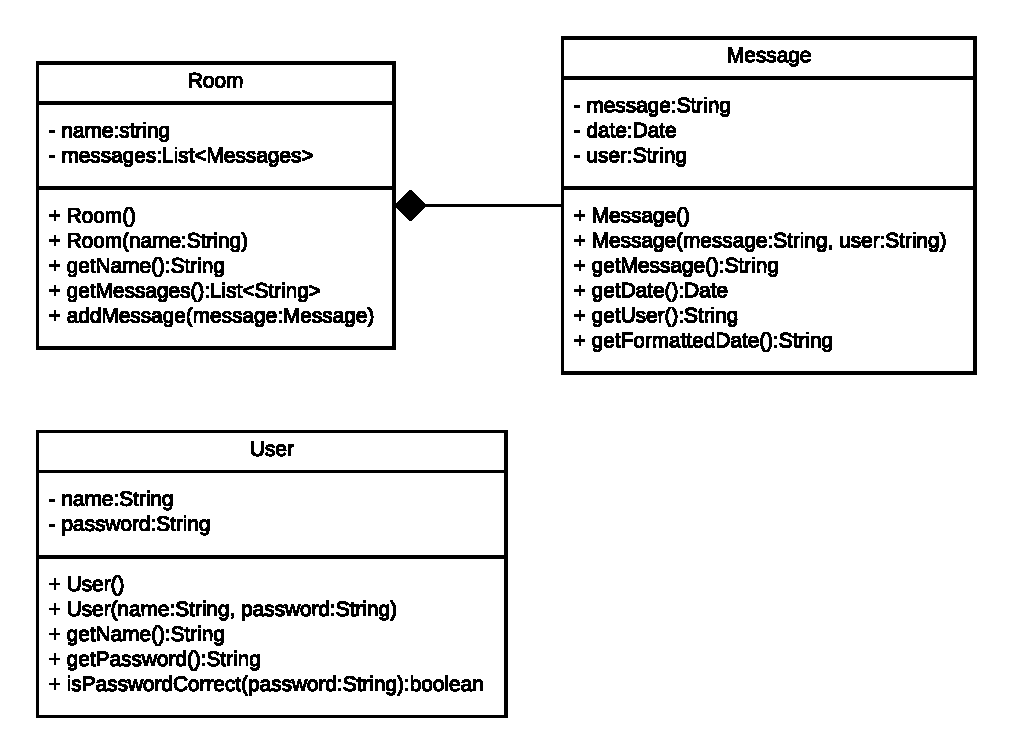
\includegraphics[scale=0.8]{images/03_impl/models}
\caption{Used models for the chat system}
\label{fig:03_impl_models_models}
\end{figure}
% Explain Figure
\Fig{fig:03_impl_models_models} shows all models used in the implementation of the chat system.
% Room and message
A \texttt{Room} model exists, which represents a room where users can chat with each other. Therefore, multiple messages are saved in a \texttt{Room}. A \texttt{Message} model represents a message sent by any user in a specific room. Each \texttt{Message} is identified by its message-text, the name of the user, and the date when it was sent.
% User
Each user is represented by a \texttt{User} model. This model is identified by the username and the password.


% ==============
% ==============
\subsection{Object Stores}\label{subsec:03_impl_objstores}
% Why
As is mentioned in \Sec{subsec:02_design_datastorage}, a custom store is needed to save models introduced in \Sec{subsec:03_impl_models}.

Therefore, the following stores are being implemented:
\begin{itemize}
\item \texttt{UserStore}, saves \texttt{User} models
\item \texttt{RoomStore}, saves \texttt{Room} models
\end{itemize}
% Store functionality
Because a user and room can only exist once, a \texttt{Set}\footnote{Set (Java Platform SE 8) - \url{https://docs.oracle.com/javase/8/docs/api/java/util/Set.html}} data structure is used to save both \texttt{Users} and \texttt{Rooms}. Furthermore, a store needs to provide the functionality to add an object to the store, get all objects from the store, or a specific one, and check if an object has already been added to the store.


% Abstract class
Therefore, an abstract class called \texttt{ObjectsStore} is implemented, which implements the previously mentioned functionalities.
% Generics
The \texttt{ObjectStore} uses generics to implement the properties and methods. The \texttt{UserStore} and \texttt{RoomStore} implement the \texttt{ObjectStore} class and set the model (\texttt{User} and \texttt{Room}, respectively) for the generic type.
% Lifetime
The lifetime of an object saved to a store is equal to the lifetime of the running webserver. As long as the webserver is running, the objects are saved to memory. If the webserver gets shut down, all rooms and messages are being removed from the memory.
% Lifetime of user
Except for the \texttt{UserStore}, which reads all \texttt{User} models from a text file, and writes newly created Users to the same file. Therefore, when the server restarts, all previously added \texttt{User} models are available again.

% Singleton pattern
To make the same set of Users, and Rooms available for each single servlet instance, the singleton pattern is used for the stores. This ensures, that all servlets work with the same set of \texttt{Users} and \texttt{Rooms}. An example of the singleton pattern usage is shown in \Lst{lst:03_impl_objstores_singleton}.
% Singleton example
\begin{lstlisting}[label=lst:03_impl_objstores_singleton, caption=Example usage of the singleton pattern, language=java]
Set<Room> rooms = RoomStore.getInstance().getAll();
\end{lstlisting}


% ==============
% ==============
\subsection{Servlets}\label{subsec:03_impl_servlets}
Each route introduced in \Sec{subsec:02_design_routes}, is implemented using a servlet. The following servlets are needed for this architecture:
\begin{itemize}
\item \texttt{AuthLoginServlet}
\item \texttt{AuthLogoutServlet}
\item \texttt{LoginServlet}
\item \texttt{UserPageServlet}
\item \texttt{RoomServlet}
\item \texttt{RoomCreateServlet}
\item \texttt{AdminServlet}
\end{itemize}
% Views
Most of the mentioned servlets own a specific view (a \texttt{JSP} file) which is saved in \path{Chat/src/main/webapp/views}.
%
\Lst{lst:03_impl_servlets_includeview} shows, how a servlet forwards a request to a specific view.
\begin{lstlisting}[label=lst:03_impl_servlets_includeview, caption=Forward a request to a view, language=java]
this.getServletContext()
  .getRequestDispatcher("/views/room/RoomCreate.jsp")
  .forward(request, response);
\end{lstlisting}


\subsubsection{Authentication}\label{subsubsec:03_impl_servlets_auth}
For authentication, the \texttt{AuthLoginServlet} and the \texttt{AuthLogoutServlet} are created.
% Login
The \texttt{AuthLoginServlet} requires a \texttt{POST} request and validates the request accordingly. If the given username and password are valid credentials (the user with the given name exists, and the password is correct), the \texttt{AuthLoginServlet} creates a new \texttt{HTTPSession}, sets the active user, and the attribute \texttt{is\_authenticated} to \texttt{true}. This property is important for the \texttt{AuthFilter} introduced in \Sec{subsubsec:03_impl_filters_auth}. After that, the \texttt{AuthLoginServlet} redirects the user to the \textit{User-Page}.
% Whre does the data come from
The users are received using the \texttt{getUser} method of the \texttt{UserStore}.
% Admin
However, the admin user is not stored in the \texttt{UserStore}. If the username is equal to \texttt{admin}, the \texttt{AuthLoginServlet} checks if the password is equal to the init property \texttt{AdminPassword}, which is set in the \texttt{web.xml} (equals to \texttt{root}).
% Invalid credentials
If the \texttt{POST} request is invalid (no username and password set), the \texttt{AuthLoginServlet} sends a \texttt{400 - Bad Request} HTTP error. Otherwise, if the request is valid, but the credentials are invalid (wrong username or wrong password), the \texttt{AuthLoginServlet} redirects back to the \textit{Login-Page}.

% Logout
To log out, the \texttt{AuthLogoutServlet} exists. If a \texttt{GET} request is made from an active user, it invalidates the \texttt{HTTPSession} and redirects the user to the \textit{Login-Page}.


\subsubsection{Login}\label{subsubsec:03_impl_servlets_login}
% Figure
\begin{figure}[h]
\centering
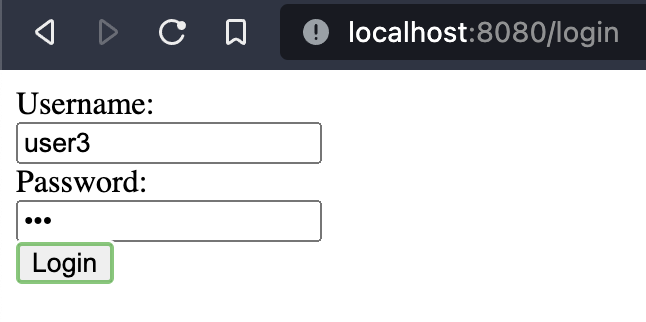
\includegraphics[scale=0.5]{images/03_impl/login/login_form}
\caption{The login HTML form}
\label{fig:03_impl_servlets_login_form}
\end{figure}
% Explain figure
\Fig{fig:03_impl_servlets_login_form} shows the \textit{Login-Page}. It consists of a single HTML form that sends a \texttt{POST} request to the \texttt{AuthLoginServlet} (introduced before in \Sec{subsubsec:03_impl_servlets_auth}) consisting of the username and the corresponding password.


\subsubsection{User}\label{subsubsec:03_impl_servlets_user}
% Figure
\begin{figure}[h]
\centering
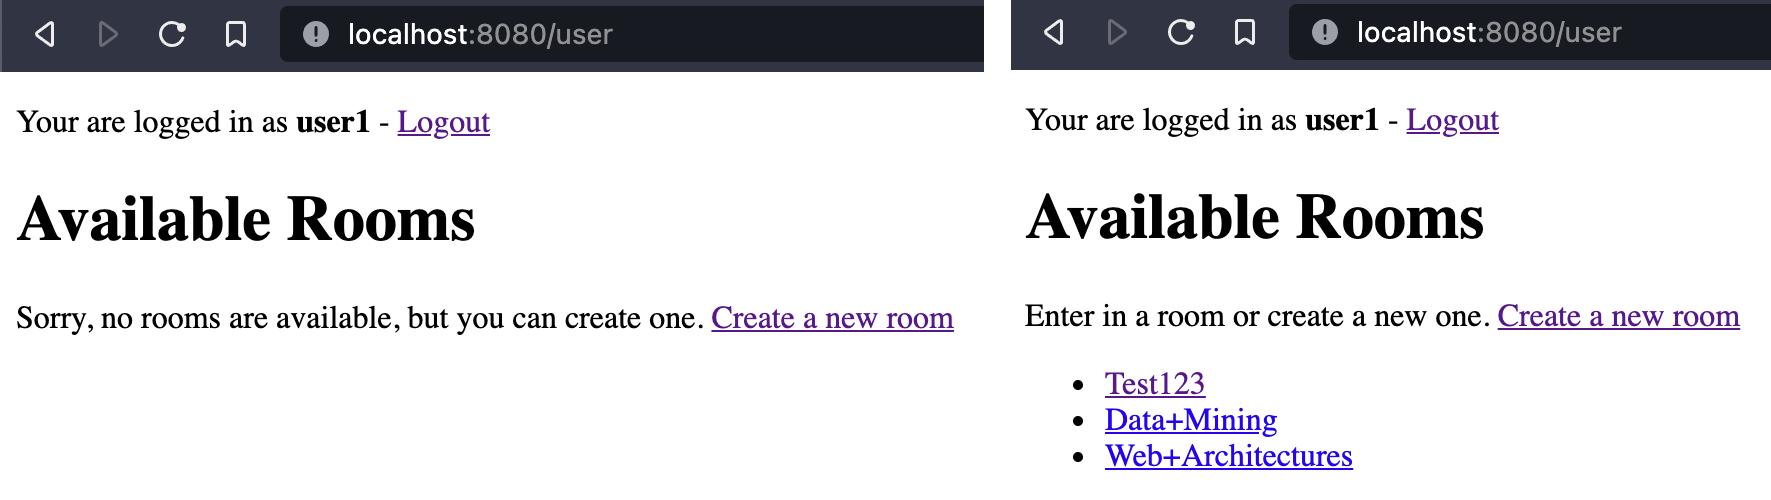
\includegraphics[scale=0.2]{images/03_impl/user/userpage_before_after}
\caption{The \textit{User-Page} with the empty message and available rooms}
\label{fig:03_impl_servlets_user_beforeafter}
\end{figure}
% Explain figure
\Fig{fig:03_impl_servlets_user_beforeafter} shows the \textit{User-Page}. It is shown that the \textit{User-Page} lists all available rooms, otherwise a message if no rooms exist.
% How
The view reads all available rooms from the \texttt{RoomStore} (introduced in \Sec{subsec:03_impl_objstores}) and uses a \texttt{for} loop to list the rooms as clickable links in a \texttt{ul} element, which is shown in \Lst{lst:03_impl_servlets_user}.
\newpage
% List rooms
\begin{lstlisting}[label=lst:03_impl_servlets_user, caption=List all available rooms, language=html]
<%@ page import="java.util.Set" %>
<%@ page import="it.unitn.disi.webarch.chat.helper.RoomStore" %>
<%@ page import="it.unitn.disi.webarch.chat.models.room.Room" %>
<%
    Set<Room> rooms = RoomStore.getInstance().getAll();
%>
...
<body>
<ul>
  <% for(Room room: rooms) { %>
    <li><a href="<% request.getContextPath(); %>/room/<%= room.getName() %>"><%= room.getName() %></a></li>
  <% } %>
</ul>
</body>
\end{lstlisting}


\subsubsection{Create Room}\label{subsubsec:03_impl_servlets_createroom}
% Figure
\begin{figure}[h]
\centering
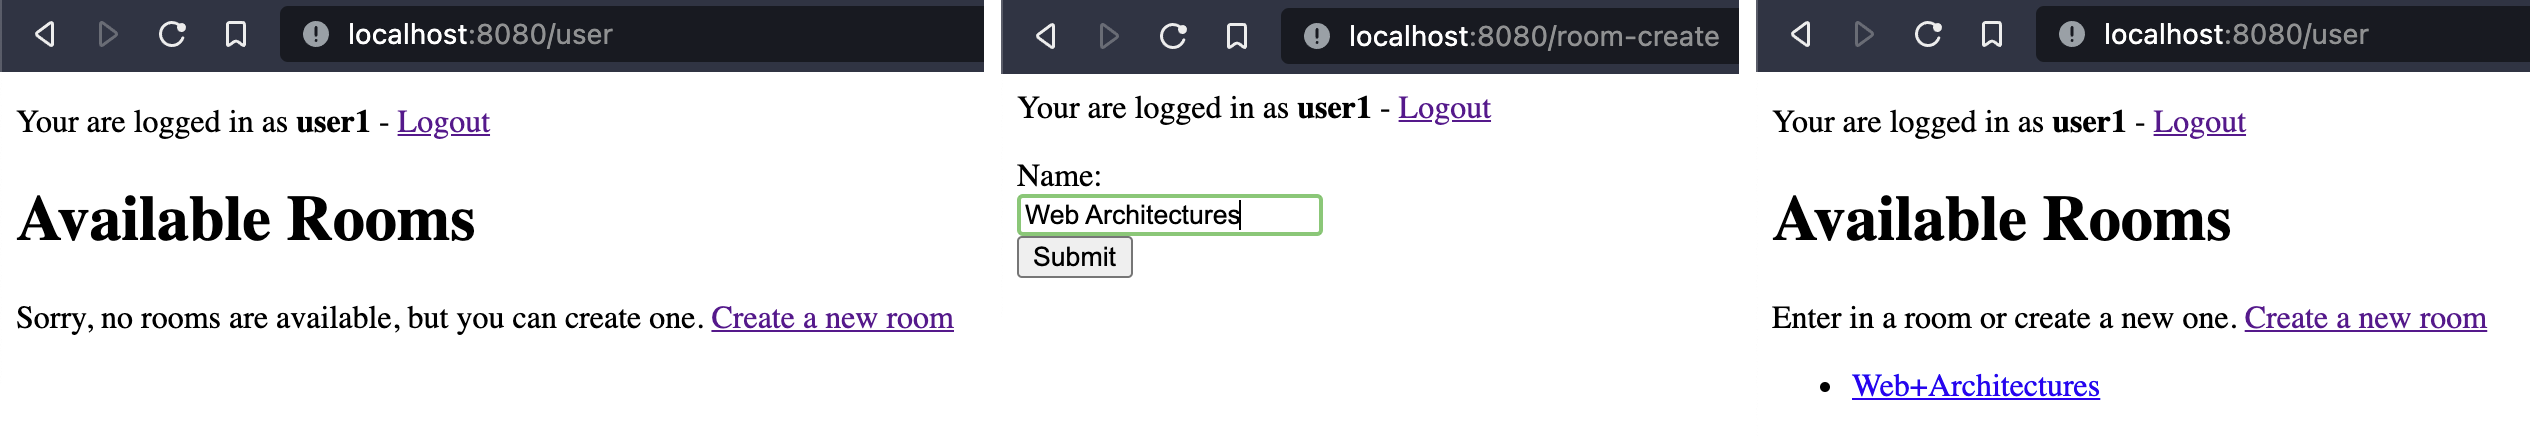
\includegraphics[scale=0.15]{images/03_impl/create-room/create-room}
\caption{Procedure of creating a new room}
\label{fig:03_impl_servlets_createroom_create}
\end{figure}
% Explain figure
The \texttt{RoomCreateServlet} includes a view that presents an HTML form to the user. The user can set a room name and submit the form as a \texttt{POST} request to itself.
% The post request
After a \texttt{POST} request has been received, the \texttt{RoomCreateServlet} creates a new instance of the \texttt{Room} model and adds the \texttt{Room} to the \texttt{RoomStore}. After a room has been created successfully, the user will be redirected to the \textit{User-Page}. This procedure is illustrated in \Fig{fig:03_impl_servlets_createroom_create}, where the room \textit{Web Architectures} is being created.
% Encoding
Additionally, the \texttt{RoomCreateServlet} encodes the name of a room using \texttt{URLEncoder.encode(ROOM\_NAME, "UTF-8")}. This is necessary because the user is allowed to use special characters like whitespaces in the room name. \Fig{fig:03_impl_servlets_createroom_create} also shows, how the room name has been encoded. The example shows that the name \textit{Web Architectures} has been encoded to \textit{Web+Architectures}.


\newpage
\subsubsection{Room}\label{subsubsec:03_impl_servlets_room}
% Figure
\begin{figure}[h]
\centering
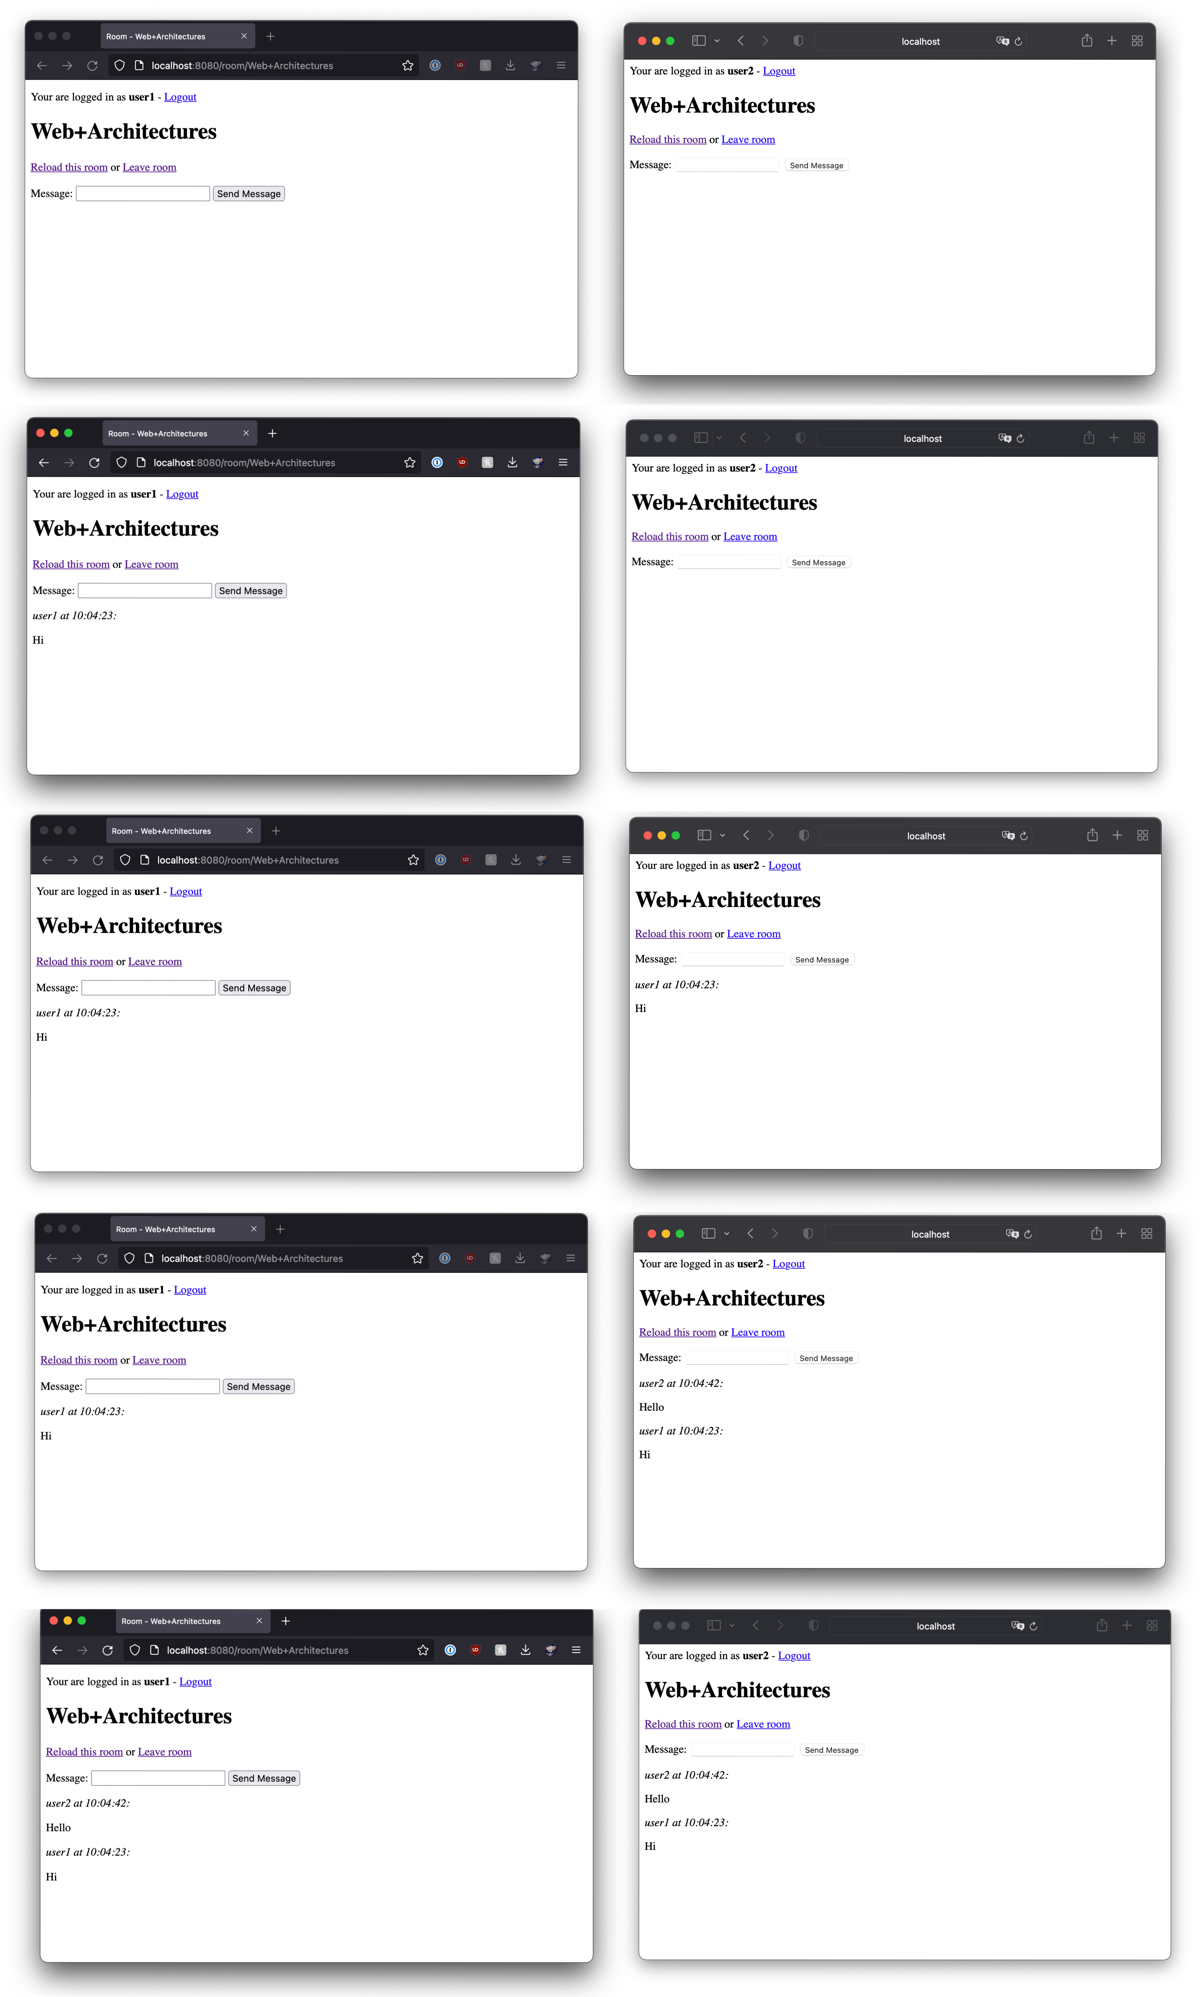
\includegraphics[scale=0.25]{images/03_impl/room/chat_all_steps}
\caption{Chat interaction between two different users in a room}
\label{fig:03_impl_servlets_admin_chat}
\end{figure}
% Explain figure
In a \textit{Room-Page}, multiple users can chat with each other, which is shown in \Fig{fig:03_impl_servlets_admin_chat}.
% The view
The \texttt{RoomServlet} owns a view called \texttt{Room.jsp}, which shows an HTML form, and lists all messages of the active Room.

% The active room
The active room is set as a Java Bean in the request. Therefore, the \texttt{JSP} view can access the model of the active room via \texttt{jsp:getProperty}. Then, all messages which belong to the active room can be received via the \texttt{getMessages()} method of a \texttt{Room} model and can be listed in a \texttt{ul} element using a \texttt{for} loop. \Lst{lst:03_impl_servlets_room_bean} shows the implementation, how messages are listed in the room view.
% The listing
\begin{lstlisting}[label=lst:03_impl_servlets_room_bean, caption=List messages for a specific room, language=html]
<%@ page import="java.util.List" %>
<%@ page import="it.unitn.disi.webarch.chat.models.room.Message" %>
<jsp:useBean id="activeRoom" class="it.unitn.disi.webarch.chat.models.room.Room" scope="request" />
...
<body>
<%
List<Message> messages = activeRoom.getMessages();
for(Message message: messages) {
%>
  <div>
    <p><em><%= message.getUser() %> at <%= message.getFormattedDate() %>:</em></p>
    <p><%= message.getMessage() %></p>
  </div>
<% } %>
</body>
\end{lstlisting}

% Send messages
The HTML form sends a \texttt{POST} request to itself. The request consists of an attribute called \texttt{message}, which is the message text of the user. After a \texttt{POST} request has been made, the \texttt{RoomServlet} constructs a new \texttt{Message} model, using the message text received from the \texttt{POST} request, and the username of the active user which is saved in the HTTP session. After that, the newly created \texttt{Message} model is added to the active \texttt{Room} model via the \texttt{addMessage} method. Finally, the page gets reloaded using the \texttt{doGet} method of the servlet. If the request is not valid (no room requested), the \texttt{RoomServlet} responds with a \texttt{400 - Bad Request} HTTP error. Otherwise, if the requested room does not exist, the \texttt{RoomServlet} responds with a \texttt{404 - Not Found} HTTP error.

% Reload
To update newly created messages, the view reloads itself every 15 seconds using \texttt{<meta http-equiv="refresh" content="15">}.


\newpage
\subsubsection{Admin}\label{subsubsec:03_impl_servlets_admin}
% Figure
\begin{figure}[h]
\centering
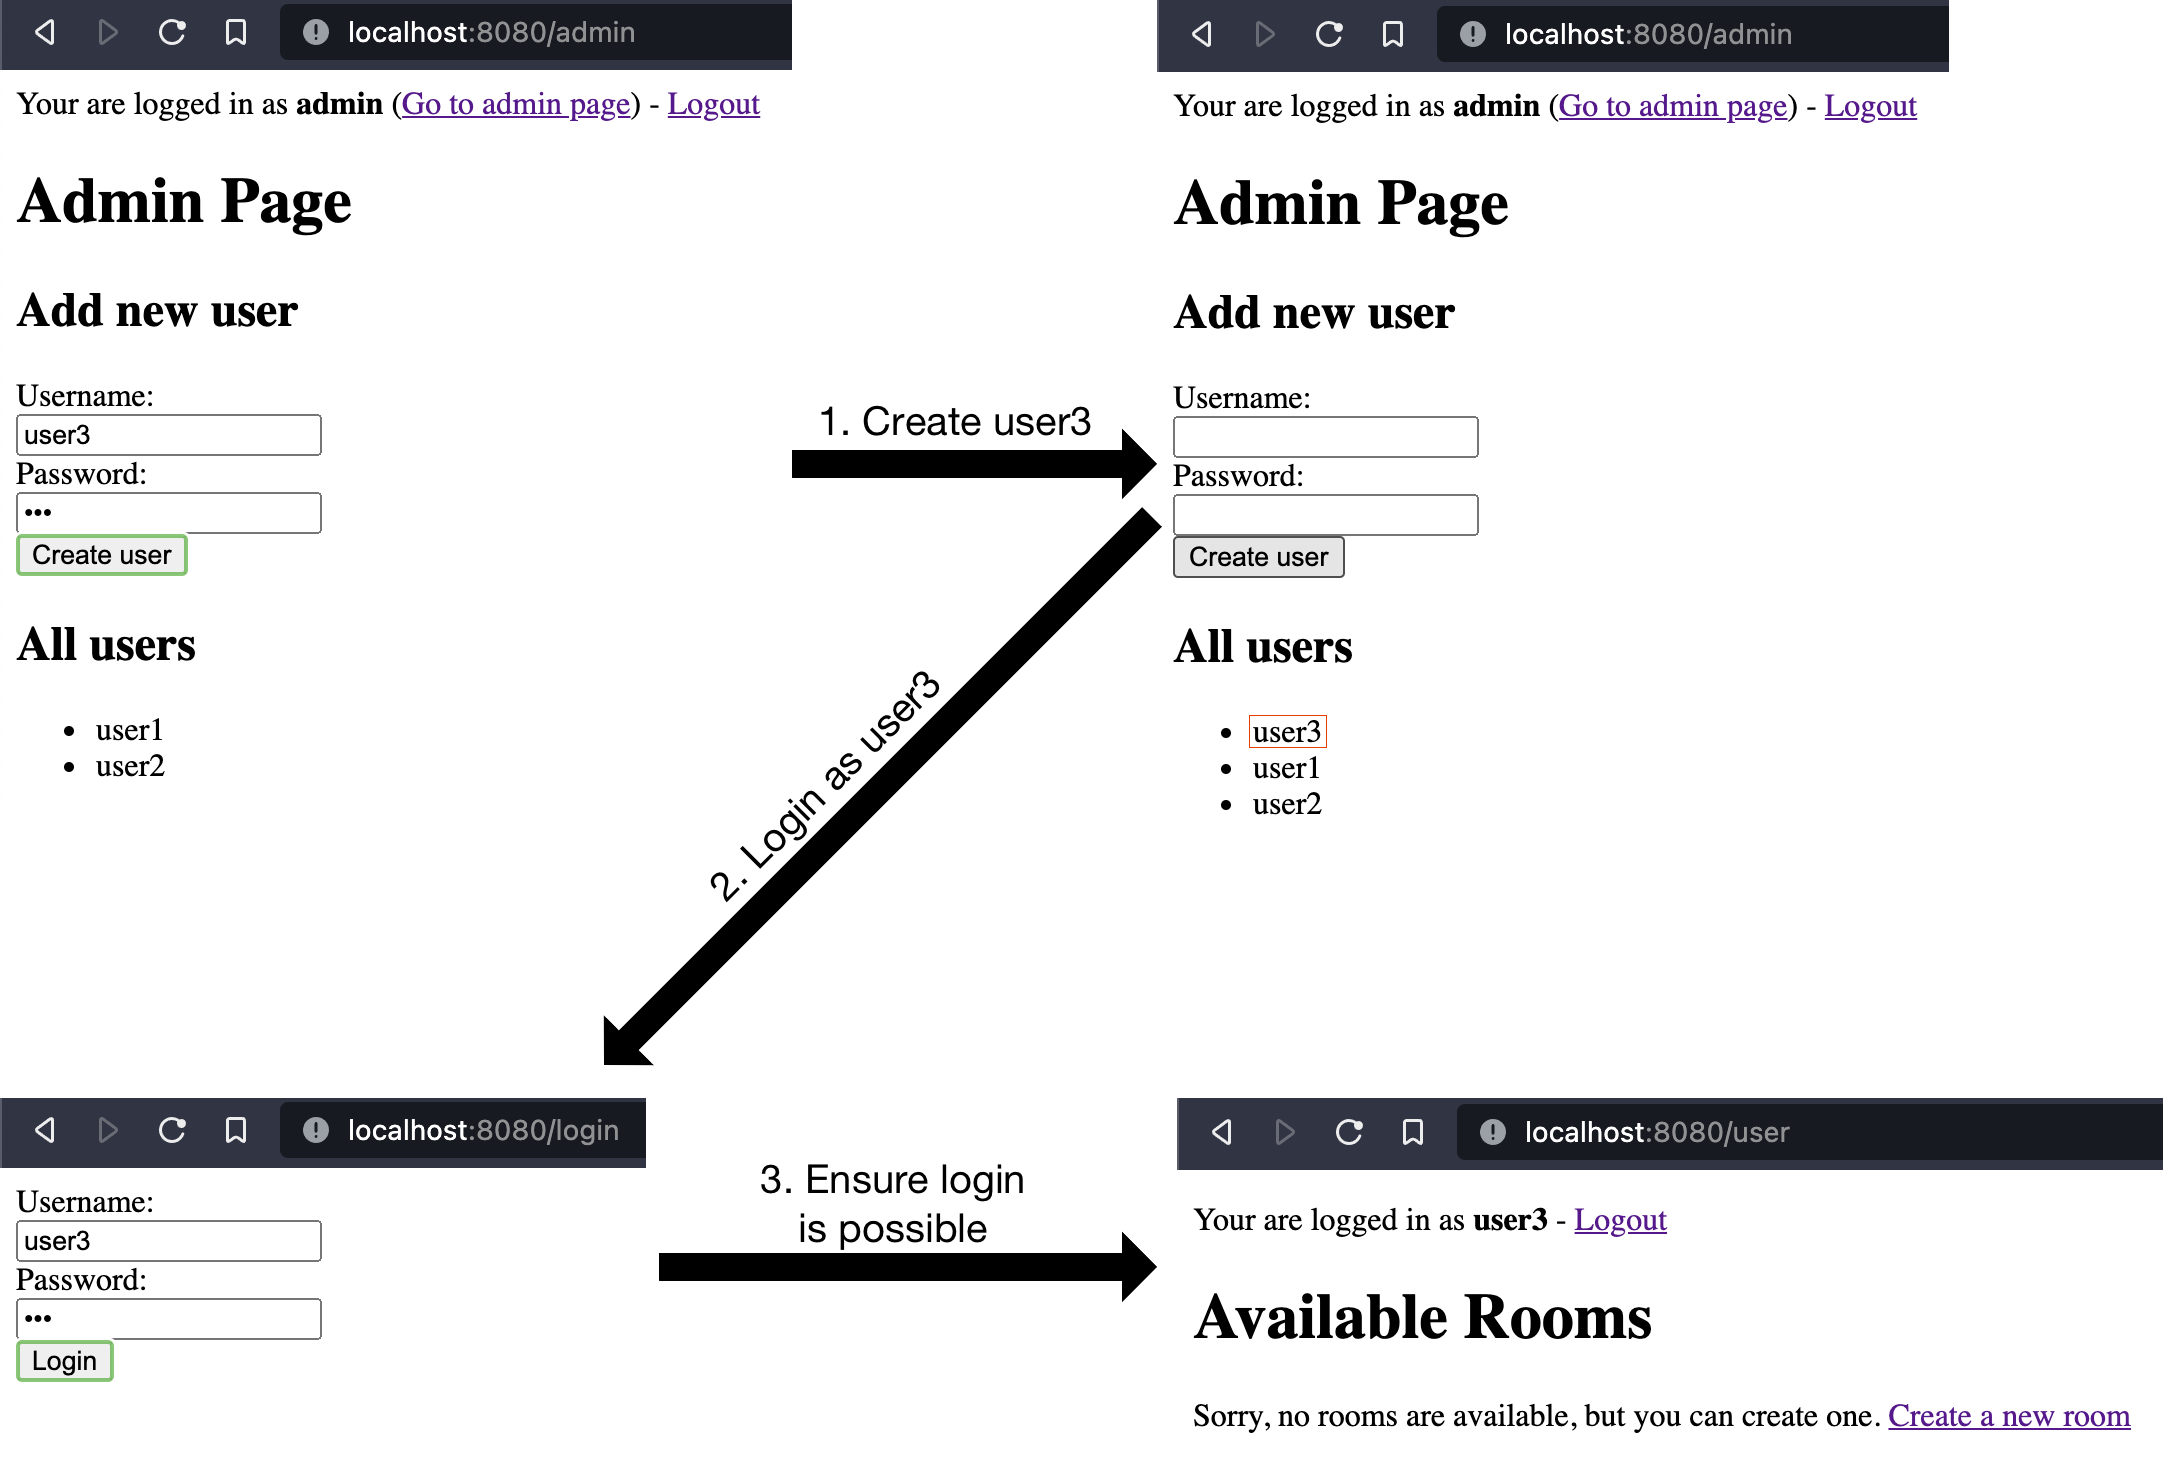
\includegraphics[scale=0.2]{images/03_impl/admin/create_user_all}
\caption{Creation-process of \textit{user3}}
\label{fig:03_impl_servlets_room_createall}
\end{figure}
% Explain figure
\Fig{fig:03_impl_servlets_room_createall} illustrates the successful creation process of a user.
% HTML for
The admin can fill out the HTML form of the \textit{Admin-Page}. After clicking submit, it will send the data (\texttt{username} and \texttt{password}) via a \texttt{POST} request to itself.
% Servlet
The \texttt{AdminServlet}, validates the \texttt{POST} request attributes and checks if the user already exists. If the user does not exist, the user will be added via the \texttt{addUser} method of the \texttt{UserStore}. As mentioned in \Sec{subsec:03_impl_objstores}, the \texttt{UserStore} will write the user to the \texttt{users.txt} file.
% Check credentials
To check if the given credentials are valid, the \texttt{AdminServlet} checks if the given \texttt{username} and \texttt{password} are not \texttt{null}. Otherwise, the \texttt{AdminServlet} will respond with a \texttt{400 - Bad Request} HTTP error. Additionally, the \texttt{AdminServlet} checks if the length of the \texttt{username} and \texttt{password} is bigger than 0 and if the \texttt{username} does not equal \textit{admin}. If one condition is not true, the \texttt{AdminServlet} executes the \texttt{doGet} method to reload itself.


% ==============
% ==============
\subsection{Banner}\label{subsec:04_impl_banner}
% The banner
As mentioned in \Sec{subsec:02_design_routes}, a \textit{Banner} is included on each page.
% No servlet
The \textit{Banner} only consists of a \texttt{JSP} file. It shows the name of the active user and a link to the logout route.
% Admin
Additionally, if the active user is the \textit{admin} user, the \textit{Banner} presents a link to the \textit{Admin-Page}.
% Figure
\Fig{fig:04_impl_banner_banner} shows the different \textit{Banner} for a normal user, and the \textit{admin} user for the \textit{User-Page}.
% Figure
\begin{figure}[h]
\centering
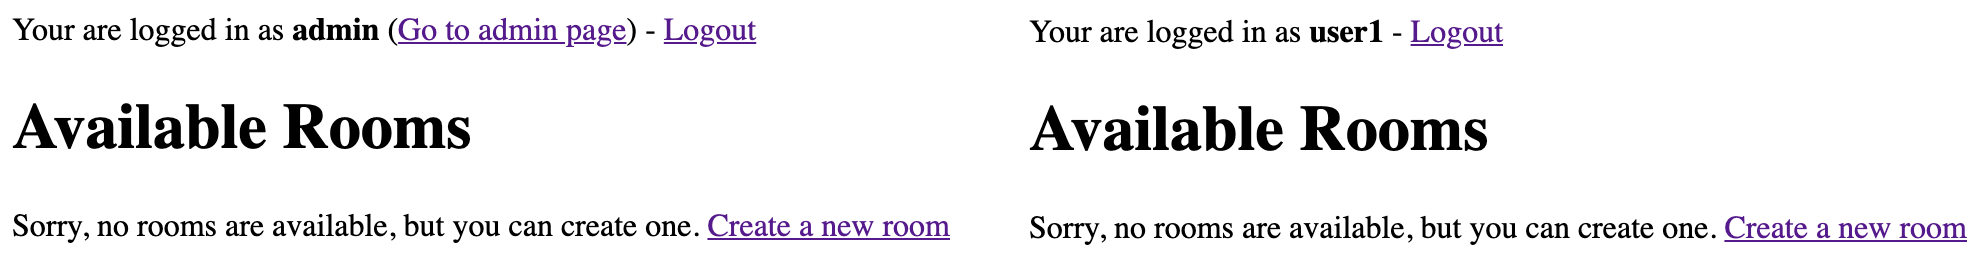
\includegraphics[scale=0.2]{images/03_impl/banner/banner}
\caption{Different Banner for different users}
\label{fig:04_impl_banner_banner}
\end{figure}


% ==============
% ==============
\subsection{Filters}\label{subsec:03_impl_filters}
% Why
Because users have to authenticate to access rooms and write messages, filters are needed to check if a user is authenticated.
% Admin
Additionally, as mention in \Sec{subsubsec:02_design_routes_admin}, only the \textit{admin} user is allowed to access the \textit{Admin-Page}. Therefore, an additional filter is needed which ensures this behavior.
% Which filter
To conclude these requirements, the following filters are implemented:
\begin{itemize}
\item \texttt{AuthFilter}
\item \texttt{AdminFilter}
\end{itemize}


\subsubsection{Authentication}\label{subsubsec:03_impl_filters_auth}
% What it does
As mentioned before, the chat system is only available for authenticated users. Therefore, a filter called \texttt{AuthFilter} checks if a request to a route, described in \Sec{subsec:02_design_routes}, has been made by an authenticated user.
% How
The \texttt{AuthFilter} checks if the session attribute \texttt{is\_authenticated} is set to \texttt{true}. This attribute is set by the \texttt{AuthLoginServlet} after a successful login, described in \Sec{subsubsec:03_impl_servlets_auth}.
% Otherwise
Otherwise, if a session does not exist or the \texttt{is\_authenticated} attribute is not set to \texttt{true}, the \texttt{AuthFilter} redirects the client to the \textit{Login-Page}. \Fig{fig:03_impl_filters_auth_redirect} shows the login HTML form after an unauthorized request has been made to the \textit{User-Page}.
% Figure
\begin{figure}[h]
\centering
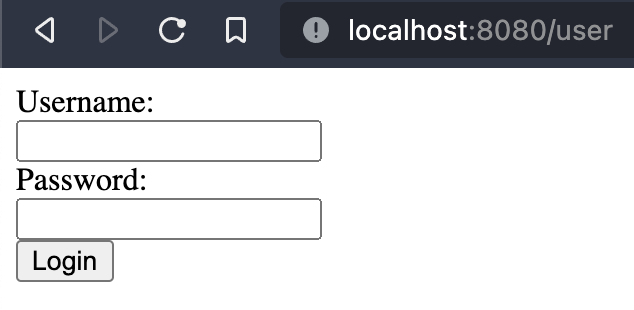
\includegraphics[scale=0.4]{images/03_impl/auth-filter/redirect}
\caption{Redirect to the \textit{Login-Page}}
\label{fig:03_impl_filters_auth_redirect}
\end{figure}


\newpage
\subsubsection{Admin}\label{subsubsec:03_impl_filters_admin}
% What
The \texttt{AdminFilter} checks if a request has been made to the \textit{Admin-Page}. If the request was made by an authenticated user, and the name of the user is equal to \textit{admin}, the filter redirects the user to the \textit{Admin-Page}.
% Otherwise
Otherwise, as illustrated in \Fig{fig:03_impl_filters_admin_forbidden}, the \texttt{AdminFilter} sends a \texttt{403 - Forbidden} HTTP error response.
% Figure
\begin{figure}[h]
\centering
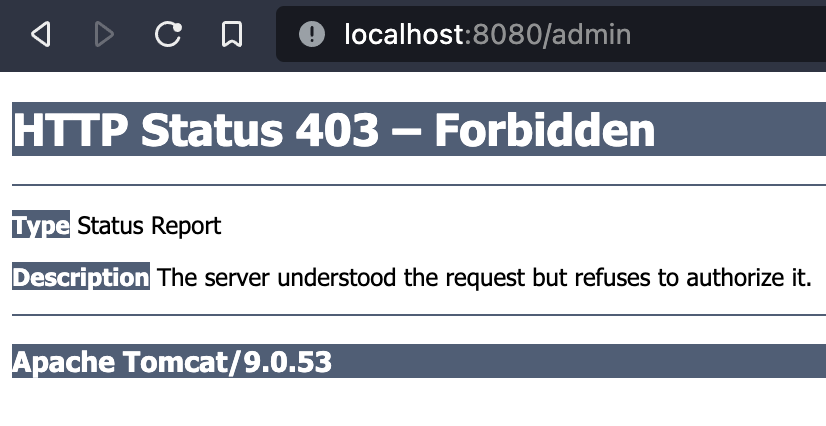
\includegraphics[scale=0.4]{images/03_impl/admin-filter/forbidden}
\caption{\texttt{403 - Forbidden} HTTP error response}
\label{fig:03_impl_filters_admin_forbidden}
\end{figure}
